\documentclass{standalone}
\usepackage{tikz}
\usetikzlibrary{shapes.geometric, arrows, positioning, fit, backgrounds, calc, shadows, decorations.pathmorphing}


\begin{document}
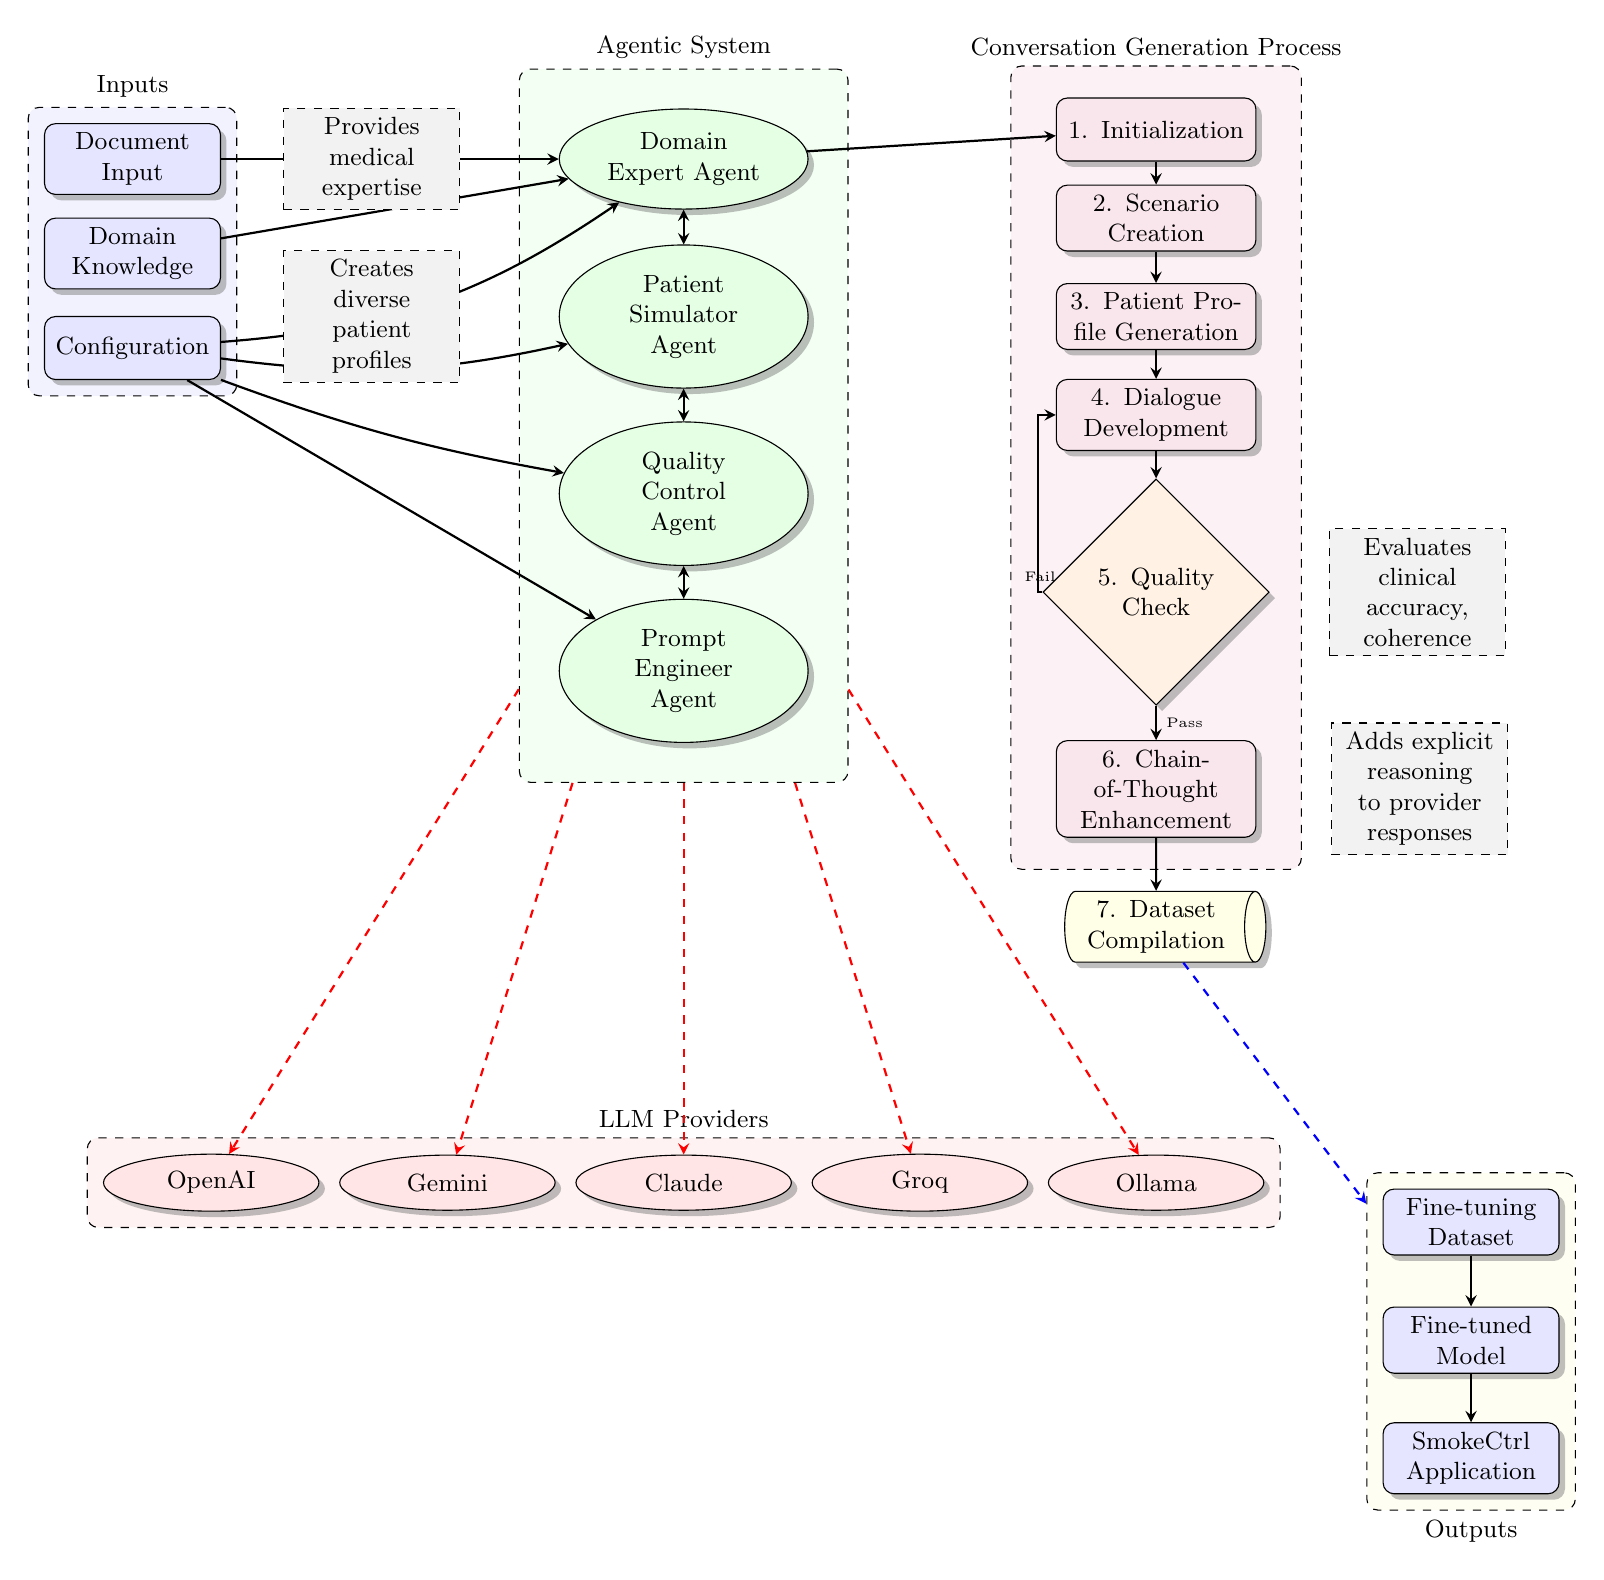
\begin{tikzpicture}[
    node distance=1.2cm,
    box/.style={rectangle, draw, text width=2cm, text centered, minimum height=0.8cm, fill=blue!10, rounded corners, drop shadow, font=\small},
    agent/.style={ellipse, draw, text width=2cm, text centered, minimum height=0.8cm, fill=green!10, drop shadow, font=\small},
    arrow/.style={thick,->,>=stealth},
    cloud/.style={ellipse, draw, text width=1.7cm, text centered, minimum height=0.7cm, fill=red!10, drop shadow, font=\small},
    database/.style={cylinder, draw, shape aspect=0.3, text width=2cm, text centered, minimum height=1cm, fill=yellow!10, drop shadow, font=\small},
    title/.style={font=\bfseries\large, align=center},
    process/.style={rectangle, draw, text width=2.3cm, text centered, minimum height=0.8cm, fill=purple!10, rounded corners, drop shadow, font=\small},
    decision/.style={diamond, draw, text width=1.8cm, text centered, minimum height=0.8cm, fill=orange!10, drop shadow, font=\small},
    note/.style={rectangle, draw, dashed, text width=2cm, text centered, minimum height=0.7cm, fill=gray!10, font=\small},
    bidir/.style={thick, <->, >=stealth},
    squiggly/.style={decorate, decoration={snake, amplitude=.3mm, segment length=1.5mm, post length=0.7mm}}
]

% Title - properly centered
% \node[title] at (0,11) {Doc2Conv Agentic Library:\\Conversation Generation Process};

% Input section
\node[box] (document) at (-7,8) {Document Input};
\node[box] (knowledge) at (-7,6.8) {Domain Knowledge};
\node[box] (config) at (-7,5.6) {Configuration};

% Agentic System
\node[agent] (domain) at (0,8) {Domain Expert Agent};
\node[agent] (patient) at (0,6) {Patient Simulator Agent};
\node[agent] (quality) at (0,3.75) {Quality Control Agent};
\node[agent] (prompt) at (0,1.5) {Prompt Engineer Agent};

% LLM Providers
\node[cloud] (openai) at (-6,-5) {OpenAI};
\node[cloud] (gemini) at (-3,-5) {Gemini};
\node[cloud] (claude) at (0,-5) {Claude};
\node[cloud] (groq) at (3,-5) {Groq};
\node[cloud] (ollama) at (6,-5) {Ollama};

% Process flow
\node[process] (init) at (6,8.375) {1. Initialization};
\node[process] (scenario) at (6,7.25) {2. Scenario Creation};
\node[process] (profile) at (6,6) {3. Patient Profile Generation};
\node[process] (dialogue) at (6,4.75) {4. Dialogue Development};
\node[decision] (quality_check) at (6,2.5) {5. Quality Check};
\node[process] (cot) at (6,0) {6. Chain-of-Thought Enhancement};
\node[database] (dataset) at (6,-1.75) {7. Dataset Compilation};

% Outputs
\node[box] (fine_tuning) at (10,-5.5) {Fine-tuning Dataset};
\node[box] (model) at (10,-7) {Fine-tuned Model};
\node[box] (app) at (10,-8.5) {SmokeCtrl Application};

% Connections between inputs and agents
\draw[arrow] (document) -- (domain);
\draw[arrow] (knowledge) -- (domain);
\draw[arrow] (config) to[bend right=15] (domain);
\draw[arrow] (config) to[bend right=10] (patient);
\draw[arrow] (config) to[bend right=5] (quality);
\draw[arrow] (config) -- (prompt);

% Connections between agents
\draw[bidir] (domain) -- (patient);
\draw[bidir] (patient) -- (quality);
\draw[bidir] (quality) -- (prompt);

% Process flow connections
\draw[arrow] (domain) -- (init);
\draw[arrow] (init) -- (scenario);
\draw[arrow] (scenario) -- (profile);
\draw[arrow] (profile) -- (dialogue);
\draw[arrow] (dialogue) -- (quality_check);
\draw[arrow] (quality_check) -- node[right, font=\tiny] {Pass} (cot);
\draw[arrow] (quality_check) -- node[above, font=\tiny] {Fail} ++(-1.5,0) |- (dialogue);
\draw[arrow] (cot) -- (dataset);

% Output connections
% \draw[arrow] (dataset) -- (fine_tuning);
\draw[arrow] (fine_tuning) -- (model);
\draw[arrow] (model) -- (app);


\begin{scope}[on background layer]
    \node[fit=(domain)(patient)(quality)(prompt), draw, dashed, rounded corners, fill=green!5, inner sep=0.5cm, label={[font=\small]above:Agentic System}, alias=agentic] {};
    \node[fit=(openai)(gemini)(claude)(groq)(ollama), draw, dashed, rounded corners, fill=red!5, inner sep=0.2cm, label={[font=\small]above:LLM Providers}, alias=llm] {};
    \node[fit=(init)(scenario)(profile)(dialogue)(quality_check)(cot), draw, dashed, rounded corners, fill=purple!5, inner sep=0.4cm, label={[font=\small]above:Conversation Generation Process}, alias=process] {};
    \node[fit=(document)(knowledge)(config), draw, dashed, rounded corners, fill=blue!5, inner sep=0.2cm, label={[font=\small]above:Inputs}, alias=inputs] {};
    \node[fit=(fine_tuning)(model)(app), draw, dashed, rounded corners, fill=yellow!5, inner sep=0.2cm, label={[font=\small]below:Outputs}, alias=outputs] {};
\end{scope}

% Connectors AFTER - now aliases are defined
\draw[thick, ->, >=stealth, dashed, red] (agentic) -- (openai);
\draw[thick, ->, >=stealth, dashed, red] (agentic) -- (gemini);
\draw[thick, ->, >=stealth, dashed, red] (agentic) -- (claude);
\draw[thick, ->, >=stealth, dashed, red] (agentic) -- (groq);
\draw[thick, ->, >=stealth, dashed, red] (agentic) -- (ollama);
\draw[thick, ->, >=stealth, dashed, blue] (dataset) -- (outputs);


% Notes - repositioned to avoid overlap
\node[note, right=0.75cm of quality_check] {Evaluates clinical accuracy, coherence};
\node[note, right=0.95
cm of cot] {Adds explicit reasoning to provider responses};
\node[note, left=1.25cm of domain] {Provides medical expertise};
\node[note, left=1.25cm of patient] {Creates diverse patient profiles};

\end{tikzpicture}
\end{document}